\chapter{Redis $\to$ Remote Dictionary Server}

\emph{Redis}, acronimo di \emph{Remote Dictionary Server}, é un archivio dati veloce, open source, in memoria e di tipo chiave-valore (\textbf{dbms NoSQL}).
Si basa su una struttura a dizionario: ogni valore immagazzinato é abbinato ad una chiave univoca che ne permette il recupero.
É stato sviluppato nel linguaggio di programmazione C, e funziona principalmente con sistemi unix based, non esiste un supporto ufficiale
per Windows.
Si basa su un modello client-server, infatti i programmi esterni dialogano con il server Redis utilizzando un socket TCP e un protocollo specifico
di tipo request-response.
Il client invia una richiesta al server attendendo la risposta sul socket ed il server elabora il comando e
invia la risposta al client.

\begin{figure}[H]
    \begin{center}
        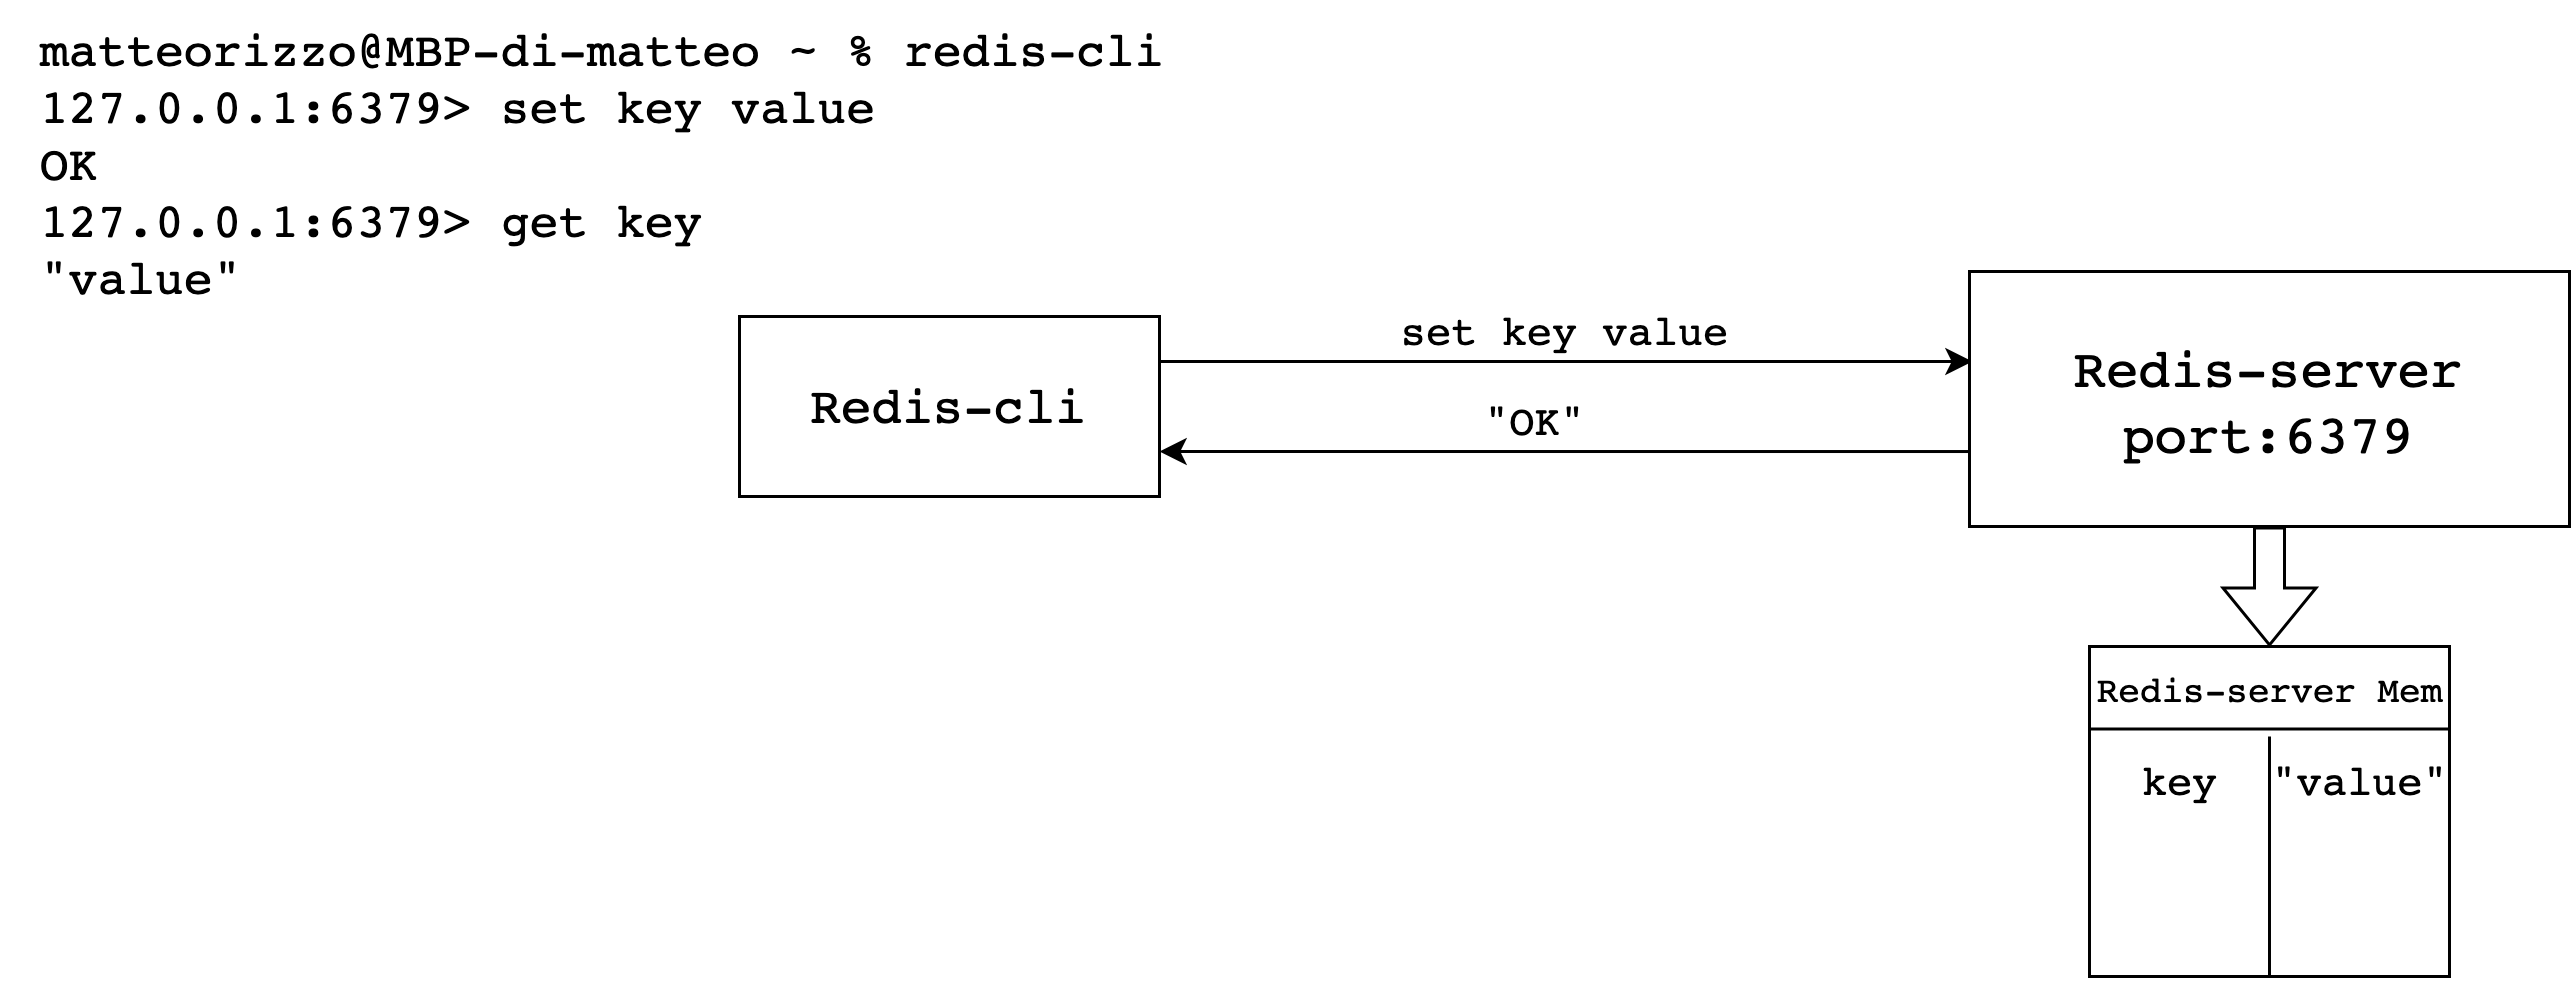
\includegraphics[width=1\textwidth]{img/redisClientServer}
    \end{center}
\caption{Modello client-server Redis}
\end{figure}

\section{Caratteristiche}
\subsection{Strutture Dati}
Una peculiarità di Redis é mettere a disposizione una grande varietá di tipi di dati associabili alle chiavi, infatti il valore archiviato
in corrispondenza di una certa chiave puó essere molto differente da un tipo semplice come la stringa ed il valore stesso puó addirittura
rappresentare una struttura dati. Inoltre, vi é una grandissima possibilitá di manipolazione grazie all'elevato numero di funzioni presenti.\\
I principali tipi di dato disponibili sono:
\begin{itemize}
    \item \textbf{Stringhe}: é il tipo piú semplice, vengono memorizzate sequenze di byte, inclusi testo, oggetti serializzati e array binari;
    sono spesso usati per la memorizzazione nella cache;
    \item \textbf{Liste}: rappresentano un elenco di stringhe indicizzate in base all'ordine di inserimento nella struttura. Possono essere
    modificate con inserimenti in testa o in coda. Vi é la possibilitá di trattare una lista come una coda (First In First Out) tramite il comando di inserimento
    \texttt{LPUSH} e il comando di prelievo \texttt{RPOP} oppure puó essere trattata come una pila (First In Last Out) tramite i rispettivi comandi 
    \texttt{LPUSH} e \texttt{LPOP};
    \item \textbf{Set}: é una raccolta non ordinata di stringhe univoche (sono chiamate \emph{membri} del set); vi é la possiblitá
    di utilizzare questa struttura dati per tenere traccia degli elementi univoci, rappresentare relazioni o eseguire operazioni di insiemi
    comuni come intersezioni, unioni e differenze;
    \item \textbf{Hash}: sono oggetti strutturati come raccolte di coppie campo(chiave)-valore. Possono essere utilizzati per rappresentare oggetti
    di base e per memorizzare raggruppamenti di contatori;
    \item \textbf{SortedSet}: sono una versione modificata dei Set. Sono anch'essi insiemi di stringhe che non ammettono duplicati ma, in piú,
    includono un valore, detto \texttt{score}, associato ad ogni elemento, in base al quale é possibile ordinare in senso ascendente o discendente i valori
    dell'insieme.
\end{itemize}
    Associati a queste strutture dati vi sono comandi specifici dedicati ad ognuna, per avere maggiori informazioni consultare
    \url{https://redis.io/docs/data-types}.

\subsection{Ambiti di utilizzo}
Redis é estremamente flessibile e grazie alla sua efficienza puó essere applicato a casi d'uso molto diversi tra loro:
\begin{itemize}
    \item \textbf{Analisi in tempo reale}: viene utilizzato come datastore in memoria per acquisire, elaborare e analizzare dati in tempo reale
    con latenze molto basse; puó essere utilizzato in modo estremamente efficace in ambito \textbf{IoT}. Infatti, si puó immaginare un sensore, o una rete di sensori, che invia
    dati in maniera continua; questa mole di dati andrà memorizzata ed elaborata con una bassa latenza.\\
    Verrá analizzato un caso reale nel quinto capitolo, in cui si mostrerà lo sviluppo di un applicativo nell'ambito
    IoT basandosi su Redis;
    \item \textbf{Caching}: puó essere utilizzato per implementare caching in memoria e ridurre la latenza di accesso ai dati. É in grado
    di servire elementi richiesti con maggiore frequenza e con tempi di risposta molto brevi. Un caso tipico é la memorizzazione
    di risultati di query complesse di database relazionali; in questo modo se l'applicazione dovrà eseguire una query svolta giá precedentemente,
    non dovrà piú comunicare con il database relazionale, ma potrà comunicare direttamente con Redis che manterrà in memoria le ultime operazioni svolte.
    \item \textbf{Chat, messaggistica e code}: grazie alle strutture dati che offre, come le liste e le hash, e strutture dati aggiuntive come pub/sub
    (in cui vi sono diversi publisher e subscriber) puó essere utilizzato per la messaggistica. Infatti vengono offerte prestazioni elevate per
    chat e flussi di commenti in tempo reale;
    \item \textbf{Classifiche di videogiochi}: é un servizio molto utilizzato per la creazione di classifiche in tempo reale. Infatti, é
    sufficiente utilizzare la struttura dati SortedSet per ottenere un elenco ordinato in base ai punteggi degli utenti. In questo modo, la classifica
    viene aggiornata simultaneamente alla variazione dei punteggi dei giocatori;
    \item \textbf{Memorizzazione}: soluzione molto utilizzata nel caso in cui occorre memorizzare e gestire dati di sessione per applicazioni su
    Internet, ad esempio profili utente, credenziali, stati di sessione e personalizzazioni specifiche per ciascun utente. Inoltre, é ideale anche
    per lo streaming di contenuti multimediali in tempo reale, in particolare per memorizzare metadati di profili utente e cronologie di visualizzazione,
    informazioni di autenticazione per milioni di utenti e file manifest con cui permettere la distribuzione di contenuti a milioni di utenti
    contemporaneamente;
    \item \textbf{Dati Geospaziali}: viene offerta una struttura per gestire dati geospaziali reali, chiamata \texttt{Geospatial},
    su vasta scala e con la massima rapiditá. È una SortedSet con uno score che viene calcolato in base alle coordinate che vengono assegnate ad un certo membro.
    Vengono offerti diversi comandi, tra cui \texttt{GEOADD} che permette di aggiungere elementi ad un indice geospaziale.
    Infatti, se consideriamo un esempio in cui stiamo tracciando un gruppo di auto basterá fare nel modo seguente:
    \begin{lstlisting}[autogobble, style=redis-cli, language=SQL]
> GEOADD auto -115.17087 36.12360 auto-p1
> GEOADD auto -115.171971 36.120609 auto-p2\end{lstlisting}
    Per aggiornare la posizione dell'auto andrá eseguito un nuovo \texttt{GEOADD} sulla stessa auto.\\
    É possibile determinare la distanza in metri tra diverse auto con il comando \texttt{GEODIST}:
    \begin{lstlisting}[autogobble, style=redis-cli, language=SQL]
> GEODIST auto auto-p1 auto-p2
  "347.0365"\end{lstlisting}
    \item \textbf{Machine Learning}: le moderne applicazioni basate sui dati necessitano di apprendimento automatico e quindi devono analizzare
    ed elaborare in modo rapido grandissime quantitá di dati di vario genere e con varie frequenze di aggiornamento.
\end{itemize}


\section{Confronto con \emph{proprietá ACID}}
Nelle basi di dati relazionali ogni transazione gode delle proprietà ACID. Nei database NoSQL non é vera questa affermazione.\\
In questa sezione si vogliono mettere in evidenza quali proprietà vengono soddisfatte da Redis e quali no.
\\
Innanzitutto, bisogna vedere in che modo sono gestite le transazioni in Redis:\\
i comandi utilizzati per le transazioni sono quattro:
\begin{itemize}
    \item \texttt{MULTI}: contrassegna l'inizio di un blocco di transazione, i comandi successivi verranno accodati per l'esecuzione
    \item \texttt{EXEC}: esegue tutti i comandi precedentemente accodati in una transazione e ripristina lo stato di connessione normale;
    \item \texttt{DISCARD}: svuota tutti i comandi precedentemente accodati in una transazione e ripristina lo stato di connessione normale;
    \item \texttt{WATCH}: contrassegna le chiavi fornite con un certo valore per eseguire un controllo condizionale al momento dell'esecuzione
    di una transazione (serve per la gestione di lock, ovvero controllo della concorrenza)
\end{itemize}

Quindi, una transazione viene eseguita in questo modo:
\begin{enumerate}
    \item inviamo il comando \texttt{MULTI}. Redis risponde \texttt{OK};
    \item digitiamo i comandi che devono far parte della transazione. Redis risponde \texttt{QUEUED}, ovvero il comando non viene eseguito
    istantaneamente ma viene messo in coda;
    \item conclusione della transazione: si puó scegliere se eseguire tutti i comandi con \texttt{EXEC} oppure annullare la transazione
    con \texttt{DISCARD}.
\end{enumerate}
\\
Di seguito viene riportato un esempio utilizzando \texttt{redis-cli} con la struttura dati lista; i comandi per gestire le liste in questo esempio
sono 2: \texttt{LPUSH}: comando per inserire un singolo elemento nella lista; \texttt{LRANGE}: comando per ottenere tutti i valori presenti nella lista

\begin{lstlisting}[autogobble, style=redis-cli, language=SQL]
> MULTI
  OK
(TX)> LPUSH listaNumeri 3
      QUEUED
(TX)> LPUSH listaNumeri 10
      QUEUED
(TX)> LPUSH listaNumeri 34
      QUEUED
(TX)> LPUSH listaNumeri 45
      QUEUED
(TX)> EXEC
      1) (integer) 1
      2) (integer) 2
      3) (integer) 3
      4) (integer) 4

> LRANGE listaNumeri 0 -1
  1) "45"
  2) "34"
  3) "10"
  4) "3"\end{lstlisting}
%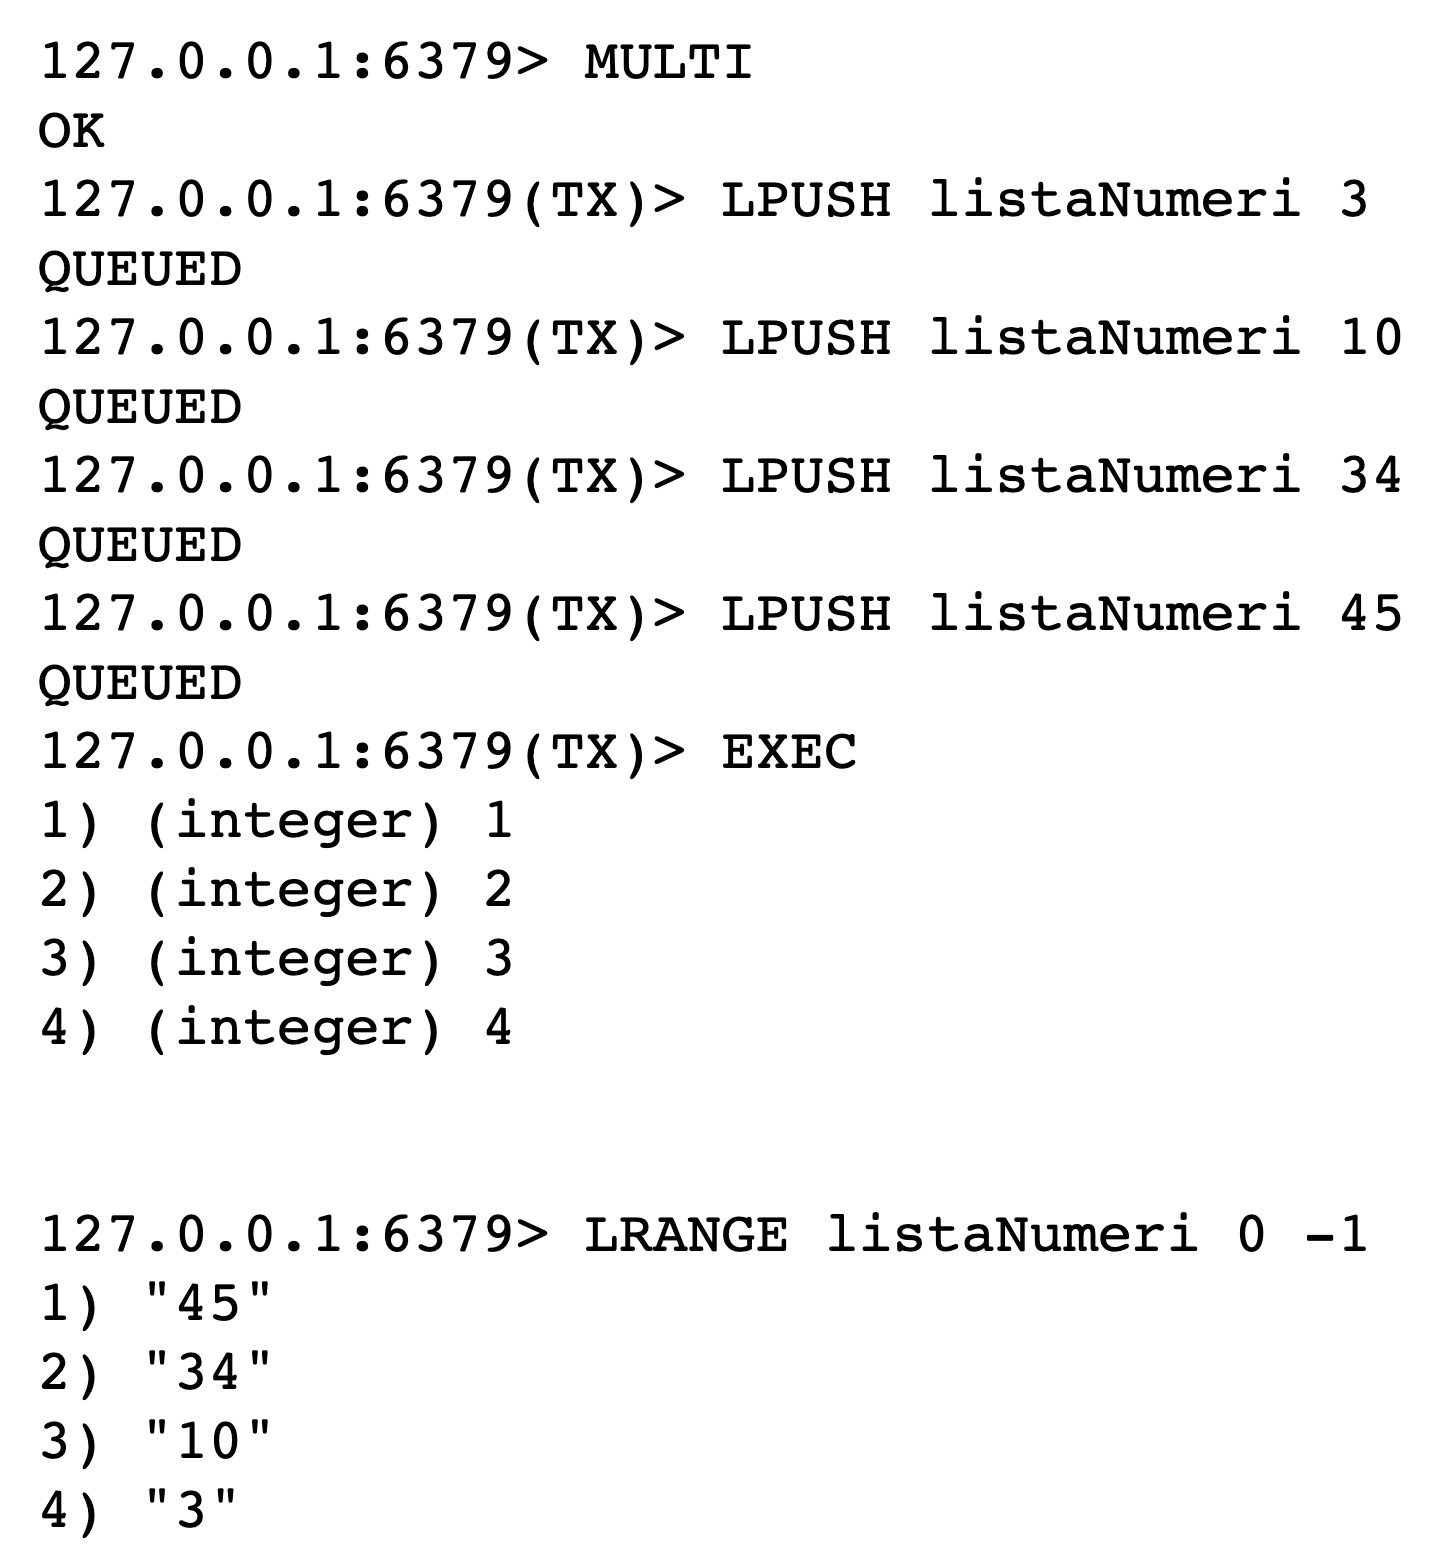
\includegraphics[width=0.7\textwidth]{img/transazioneRedis}\\
Si puó notare come l'inserimento di tutti i valori nella lista avvenga dopo il comando \texttt{EXEC}.\\
\paragraph{Quali proprietá ACID implementa Redis?}
\begin{itemize}
    \item \textbf{Atomicitá}: Redis puó avere due livelli di atomicitá:
      \begin{itemize}
          \item singola operazione: ovvero ogni singola richiesta da parte del client viene eseguita in maniera atomica dal server;
          \item transazione con operazioni multiple: come illustrato sopra con i comandi appositi;
      \end{itemize}

    \item \textbf{Isolamento}:
    Tutti i comandi in una transazione vengono serializzati ed eseguiti in sequenza. Una richiesta inviata da un altro client
    non sará mai soddisfatta nel bel mezzo dell'esecuzione di una transazione. Ció garantisce che i comandi vengano eseguiti
    come un'unica operazione isolata.\\
    Se vogliamo avere un isolamento multi-transazionale, vi é un meccanismo che riesce a fornire delle garanzie, in cui viene fatta una sorta di operazione
    di check-and-set.
    Questo meccanisco utilizza il comando \texttt{WATCH} definito precedentemente.
    Le chiavi, su cui viene definito watch, vengono continuamente monitorate per eventuali modifiche; se anche una sola chiave monitorata
    da \texttt{WATCH }viene modificata prima della \texttt{EXEC}, l'intera transazione verrá abortita.\\

    Consideriamo un esempio in pseudo-codice in cui si deve aumentare il valore di una chiave di 1.

    \begin{lstlisting}[autogobble, style=redis-cli, language=SQL]
num = GET sampleKey
num = num + 1
SET sampleKey num\end{lstlisting}

    i comandi mostrati sopra funzioneranno senza problemi purché sia presente un solo utente che esegue l'operazione in un determinato momento.\\
    Il problema si verifica nel caso in cui ci siano piú utenti che tentano di aumentare il valore della chiave contemporaneamente.
    Possiamo eliminare questo potenziale problema di race condition utilizzando il comando \texttt{WATCH} nel modo seguente:

    \begin{lstlisting}[autogobble, style=redis-cli, language=SQL]
WATCH sampleKey
num = GET sampleKey
num = num + 1
MULTI
SET sampleKey num
EXEC\end{lstlisting}

    Con questa implementazione, se si dovesse verificare una race condition ed un client modifica il valore di \texttt{sampleKey} tra il nostro
    \texttt{WATCH} e \texttt{EXEC}, la transazione verrá interrotta. Avremo bisogno di ripetere la transazione quando la race condition non sará
    piú presente.\\

    \item \textbf{Consistenza}: I vincoli di integritá sono dei concetti relazionali, quindi é difficile fare un collegamento con un database di questo tipo.
    L'unica chiave che esiste é quella primaria e deve essere univoca;
    l'integrita referenziale non é mantenuta da Redis stesso e deve essere gestita dalle applicazioni client.

    \item \textbf{persistenza (durability)}:
    l'efficienza di Redis é dovuta in buona parte al suo modo di gestire questa proprietá.
    É un database in memoria ma con possibilitá di essere persistente su disco, quindi rappresenta un compromesso in cui si ottengono
    velocitá di scrittura e lettura molto elevate con la limitazione di avere un set di dati non piú grande della memoria.
    Questo database mette a disposizione la possibilitá di scegliere tra diversi meccanismi
    offrendo l'opportunitá di salvare database
    totalmente su disco oppure no.\\
    I meccanismi, che verranno illustrati di seguito, sono:
      \begin{itemize}
          \item \textbf{RDB}
          \item \textbf{AOF}
          \item \textbf{Database in Memory}
      \end{itemize}%parlate anche dei dati salvati in cache, vantaggi/svantaggi che ne derivano
        
       \paragraph{RDB $\to$ Redis Database File:}
         Questo tipo di persistenza esegue snapshot del set di dati a intervalli specificati. Viene prodotto come risultato un file
         compatto, pertanto agevole da salvare su qualsiasi tipo di supporto. Inoltre, il recupero dei dati all'avvio del server Redis
         é molto efficiente.
         Il salvataggio dei dati viene eseguito su file ad intervalli di tempo e non con continuitá, quindi questo potrebbe essere un punto a sfavore
         nel caso di crash del sistema tra uno snapshot ed un altro con conseguente perdita dei dati.
         Conviene utilizzare questo tipo di persistenza quando si richiede un salvataggio meno oneroso per il server e si ha particolare interesse
         ad avere un backup piú comodo.

    \paragraph{AOF $\to$ Append Only File:}
    É un meccanismo di persistenza che consente al server Redis di tenere traccia e registrare ogni comando eseguito dal server.
    Vi é un file di log dove vengono aggiunti i comandi ogni volta che vengono eseguiti.
    Questo registro di comandi puó essere riprodotto all'avvio del server, ricreando il database al suo stato originale.
    Il vantaggio é che basandosi su un log scritto continuamente, non vi é il rischio di incorrere in perdite in caso di crash. Inoltre,
    il formato dei file che vengono prodotti da questa modalitá permette un recupero piú semplice in caso di corruzione.
    Peró, i file AOF risultano meno compatti e piú voluminosi rispetto a quelli in formato RDB e da ció consegue un ripristino del database
    meno rapido all'avvio. Questo meccanismo viene utilizzato quando la principale preoccupazione é la perdita di dati.\\

    É possibile utilizzare contemporaneamente AOF e RDB, e durante il ripristino del database verrá preferito l'utilizzo di file AOF, per la loro
    maggiore completezza.


    \paragraph{Database In Memory:}
    É possibile rinunciare ad entrambi i meccanismi definiti precedentemente per dare vita ad un database in memory senza persistenza su disco, risultando molto piú
    efficiente, poiché non deve piú occuparsi dei salvataggi, e puó essere utilizzato per immagazzinare dati ad uso temporaneo la cui
    perdita non risulterebbe irreparabile per il sistema.\\
    Questa modalità solitamente é quella utilizzata per fare caching, nella quale viene fissata la quantità massima di memoria utilizzabile. Quando questa sará
    colma, i dati piú vecchi verranno eliminato con una politica LRU o LFU.
\end{itemize}

\paragraph{Come configurare i diversi livelli di persistenza?\\}
Per fare ció bisogna accedere al file di configurazione del server Redis andando a modificare/cancellare dei parametri e riavviando il server,
oppure digitando \texttt{CONFIG SET ...} da CLI, con la possibilitá di avere un effetto immediato sulle modifiche apportate alla configurazione del server senza doverlo riavviare.\\
\\
Di seguito viene illustrato un esempio di modifica del file di configurazione, denominato \texttt{redis.conf}.\\
\\
RDB é l'impostazione predefinita. In particolare sono giá impostati i seguenti parametri di default:
\begin{lstlisting}[autogobble, style=redis-cli, language=SQL]
save 900 1
save 300 10\end{lstlisting}
Ció significa che viene eseguito uno snapshot dopo 900 secondi se vi é almeno 1 modifica al set di dati e dopo
300 secondi se vi sono almeno 10 modifiche al set di dati.
Di conseguenza, se si ha la necessitá di avere intervalli aggiuntivi o diversi é molto semplice andare a modificarli aggiungendo o togliendo questi parametri predefiniti.\\
\\
Al momento del salvataggio verrá visualizzato un messaggio di questo tipo nella CLI del server:
\begin{lstlisting}[autogobble, style=redis-cli, language=SQL]
10 changes in 300 seconds. Saving...
Background saving started by pid ...
DB saved on disk\end{lstlisting}\\
\\
\\
La strategia AOF viene configurata mediante due parole chiave:\\
\texttt{appendonly}, che se impostato a \texttt{yes} attiva AOF;\\
\texttt{appendfilename}, che specifica il nome del file in cui verranno salvate le operazioni.\\
\\
Per ottenere un \emph{database in memory} senza persistenza é sufficiente includere questi comandi:
\begin{lstlisting}[autogobble, style=redis-cli, language=SQL]
save ""
appendonly no\end{lstlisting}



\section{sistema distribuito}
Redis supporta una distribuzione di vari processi server su piú macchine con la possibilità di collaborazione tra di loro.
Oltre alle soluzioni proprietarie fatte su misura in base al caso d'uso specifico, Redis offre la possibilità di avere lato server un
sistema distribuito in modo piuttosto semplice ed efficiente.\\
vi sono due tipologie di sistemi distribuiti che é possibile implementare:
\begin{itemize}
    \item \textbf{Redis Master-Slave}
    \item \textbf{Redis Cluster}
\end{itemize}
Per sistemi estremamente avanzati, vi é la possibilità di fondere queste due modalità.
\subsubsection{Redis Master-Slave}
Redis puó implementare un'architettura master-slave, ovvero un noto paradigma informatico in cui un dispositivo o processo (il master)
controlla o coordina piú dispositivi o processi subordinati (gli slave).
\\
Il server Redis puó essere eseguito in due modalitá:
\begin{itemize}
    \item Modalità Master (Redis Master);
    \item Modalità Slave (Redis Slave o Redis Replica).
\end{itemize}
\\
\\
Redis Master funge da interfaccia con il mondo esterno, gestendo tutte le richieste di scrittura esterne e puó gestire anche
quelle di lettura;
ogni volta che viene apportata una modifica al database master, la modifica viene propagata ai database slave collegati al master.\\

\begin{figure}[H]
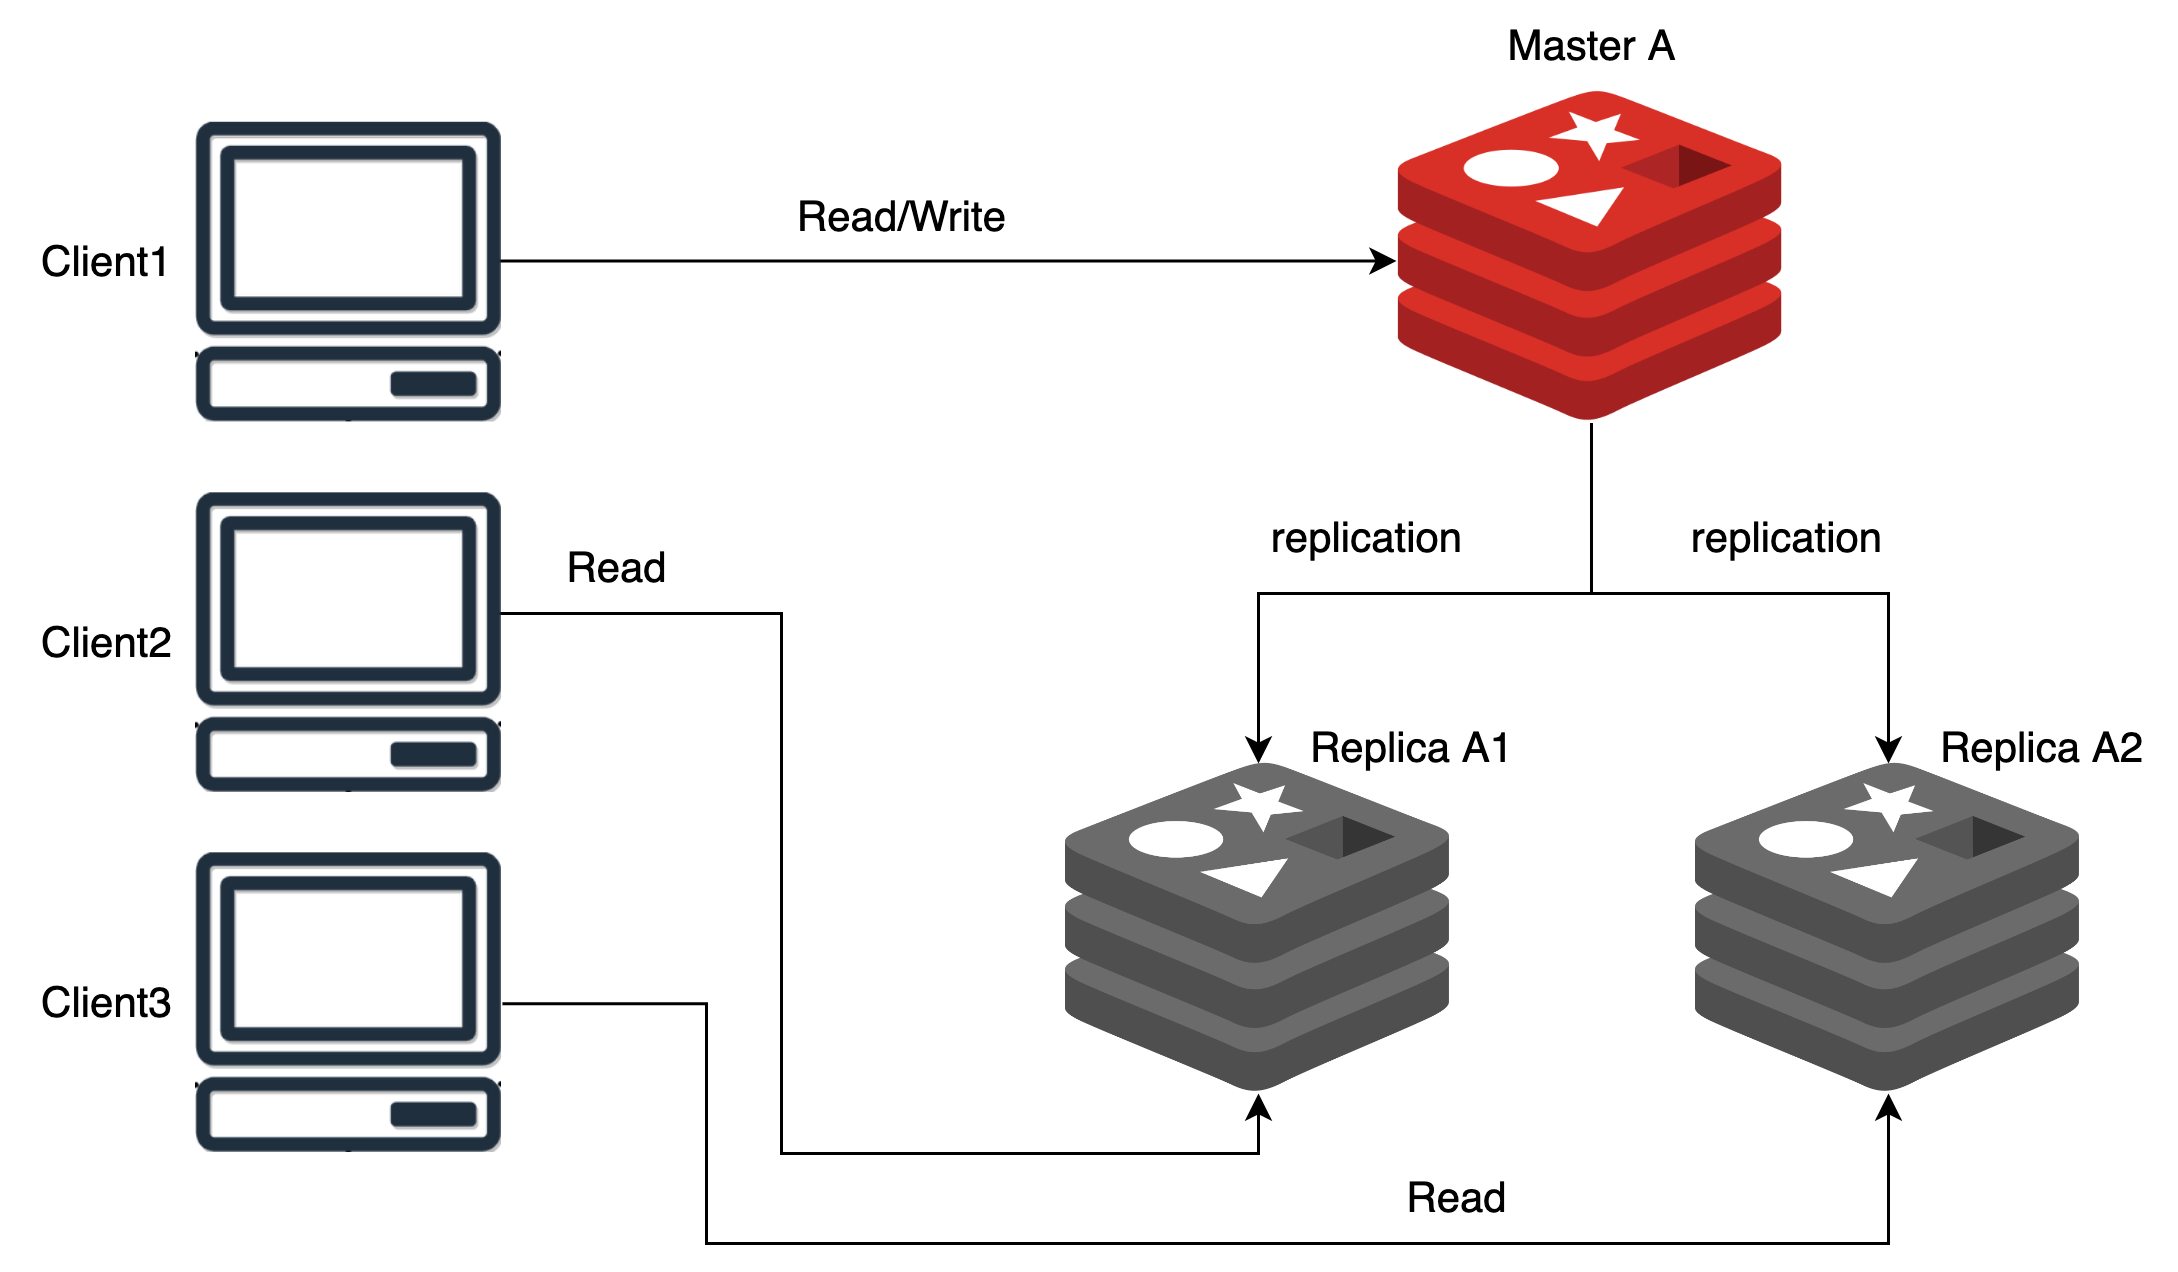
\includegraphics[width=1\textwidth]{img/masterslaveRedis}
\caption{Redis distribuito master-slave}
\end{figure}
\\
La propagazione della replica puó avvenire in due modi:
\begin{itemize}
    \item sincrona: le modifiche ai database slave avvengono apportate istantaneamente;
    \item asincrona: le modifiche vengono apportate solo a distanza di tempo, é l'impostazione predefinita poiché si adatta
    alla maggior parte dei casi d'uso di Redis.
\end{itemize}
\\
La replica master-slave é in gran parte non bloccante, il che significa che il database master puó continuare a funzionare
mentre i database slave sincronizzano i dati.
I Redis Slave saranno in grado di gestire le query utilizzando la versione non aggiornata del database, tranne che per un breve
periodo durante il quale vengono caricati i nuovi dati.

\paragraph{Come avviene il failover nel caso di guasto di Redis Master?\\}
vi sono due scelte:
\begin{enumerate}
    \item aggiungi una nuova macchina come Redis Master;
    \item rendi qualsiasi Redis Slave esistente come nuovo Redis Master.
\end{enumerate}
Il problema con l'approccio \textbf{1} é che nel momento in cui aggiungiamo una nuova macchina che fa da Master e questa sincronizzerà
tutti i dati sui vari Slaves perderemo tutti i dati.\\
L'approccio \textbf{2} é quello migliore perché lo slave esistente avrá giá tutti i dati e una volta che lo avremo impostato in modalità
Master, esso replicherà/sincronizzerà i dati su tutti gli Slaves, il che significa che non avremo una perdita di dati, o comunque
avremo una minima perdita di dati nel caso in cui il guasto del Master si sia verificato prima della sincronizzazione con gli slaves.
\\
Invece, nel caso di crash di Redis Slave le sue richieste di lettura saranno semplicemente sostituite da altri Redis Slave.

\paragraph{Teorema CAP\\}
Formulato da Eric Brewer nel 1998, afferma che se i dati vengono memorizzati in un sistema distribuito tra i nodi di una rete, solo due delle seguenti
proprietà possono essere soddisfatte contemporaneamente:
\begin{itemize}
    \item \textbf{Consistency}: le operazioni di lettura restituiscono il dato aggiornato, ovvero proveniente dall'ultima scrittura dello stesso,
    oppure un messaggio d'errore. Non bisogna confonderla con la consistenza delle proprietá ACID, infatti questa fa riferimento al valore piú aggiornato
    di un certo dato, mentre nelle proprietà ACID si fa riferimento al rispetto dei vincoli d'integritá.
    \item \textbf{Availability}: l'accesso ai dati é sempre garantito, non si ricevono mai messaggi d'errore, ma i dati restituiti non sono necessariamente
    consistenti, ovvero potrebbero non coincidere con quelli utilizzati nell'ultima operazione di scrittura degli stessi.
    \item \textbf{Partition Tolerance}: il sistema continua a funzionare nonostante alcuni messaggi vengano persi o subiscano rallentamenti
    nelle comunicazioni tra i nodi della rete.
\end{itemize}
\\
É un teorema che viene utilizzato per analizzare le dinamiche dei sistemi informativi che possiedono due o piú archivi di dati posti su
nodi distinti della rete. Quindi, la versione distribuita di Redis rientra perfettamente in questa categoria.\\
\\
Redis é un sistema \textbf{AP}, ovvero non fornisce una forte coerenza.
\paragraph{Per quale motivo?\\}
Quando Redis Master riceve una richiesta di scrittura da un cliente:
\begin{enumerate}
    \item Esegue la richiesta del cliente e manda un ack di conferma;
    \item Redis Master replica la richiesta di scrittura su uno o piú slave.
\end{enumerate}
\\
Redis Master non attende il completamento della replica sugli slave, ma esegue prima la richiesta del client.
Se supponiamo che il guasto del Master avvenga prima del completamento della replica agli Slave avremo una perdita di coerenza.\\
\\
Potremmo pensare di migliorare la coerenza con la replica sincrona, forzando prima il Redis Master a replicare e poi mandare l'ack
di conferma al client, ma questo riduce pesantemente le prestazioni di scrittura e comunque non si ha una garanzia di consistenza.
Infatti, potrebbe verificarsi lo scenario in cui uno Slave non ha ricevuto la scrittura e viene promosso a Master.


\subsubsection{Redis Cluster}
Uno dei piú grandi limiti di Redis, essendo un database in-memory, é la limitazione della memoria che un'istanza di Redis puó avere, in quanto
tutto il set di dati archiviato non deve mai superare la dimensione massima della memoria stessa.
\\
Vi é la possibilità di suddividere i dati in diverse istanze eseguite su piú server, in modo che ogni
istanza contenga solo un sottoinsieme delle chiavi; tutto questo avviene tramite l'operazione di
\textbf{sharding}, ovvero il partizionamento orizzontale.
\\
Vi sono dei compromessi da considerare: suddividendo i dati in molte istanze, nasce il problema della
ricerca delle chiavi, quindi i dati devono essere partizionati seguendo alcune regole coerenti.\\
Sono possibili diverse implementazioni per il partizionamento dei dati:
\begin{itemize}
    \item \textbf{partizionamento lato client}: i client selezionano direttamente l'istanza corretta per
    scrivere o leggere una determinata chiave;
    \item \textbf{partizionamento assistito da proxy}: i client inviano le richieste a un proxy che supporta il protocollo Redis,
    invece di inviare le richieste direttamente alle istanze Redis corrette. Il proxy si assicurerá di inoltrare le richieste
    alle istanze corrette in base allo schema di partizionamento configurato e invierà le risposte ai client.
    Il limite principale di questa implementazione é che il proxy puó diventare un "collo di bottiglia", poiché
    tutte le richieste e risposte passano per esso.
    \item \textbf{instradamento della query}: i client inviano la query a un'istanza Redis casuale e l'istanza si
    assicurerà di inoltrare la query a quella corretta.
    Il client successivamente dovrà essere reindirizzato all'istanza corretta.
\end{itemize}
In realtà, Redis Cluster utilizza una \textbf{forma ibrida di instradamento della query}, in cui il nodo casuale che viene interrogato
non inoltra la query al nodo corretto, ma reindirizza solo il client.\\

\paragraph{A che nodo assegnare una chiave?\\}
Si introduce l'idea degli \textbf{Hash Slot}, in particolare un cluster dispone di 16384 slot.
Essi vengono assegnati in maniera piú o meno equa tra i vari nodi.
Ad ogni chiave viene associato un numero, ottenuto applicando alla chiave una Hash Function chiamata \texttt{CRC16}
e facendo il modulo di 16384.
Il numero ottenuto indicherà lo slot di appartenenza, e di conseguenza, il nodo di appartenenza.
Quindi, al momento dell'inserimento/richiesta di informazioni di una chiave viene applicata questa funzione alla chiave stessa,
ed in base al numero ottenuto il client verrà reindirizzato al nodo proprietario del numero di slot ottenuto, ed eseguirà la richiesta.\\
Dopo un certo numero di interrogazioni i client riescono ad ottenere una mappatura completa di quali nodi sono proprietari di quali slot,
potendo contattare direttamente i nodi corretti.
\begin{figure}[H]
    \begin{center}
        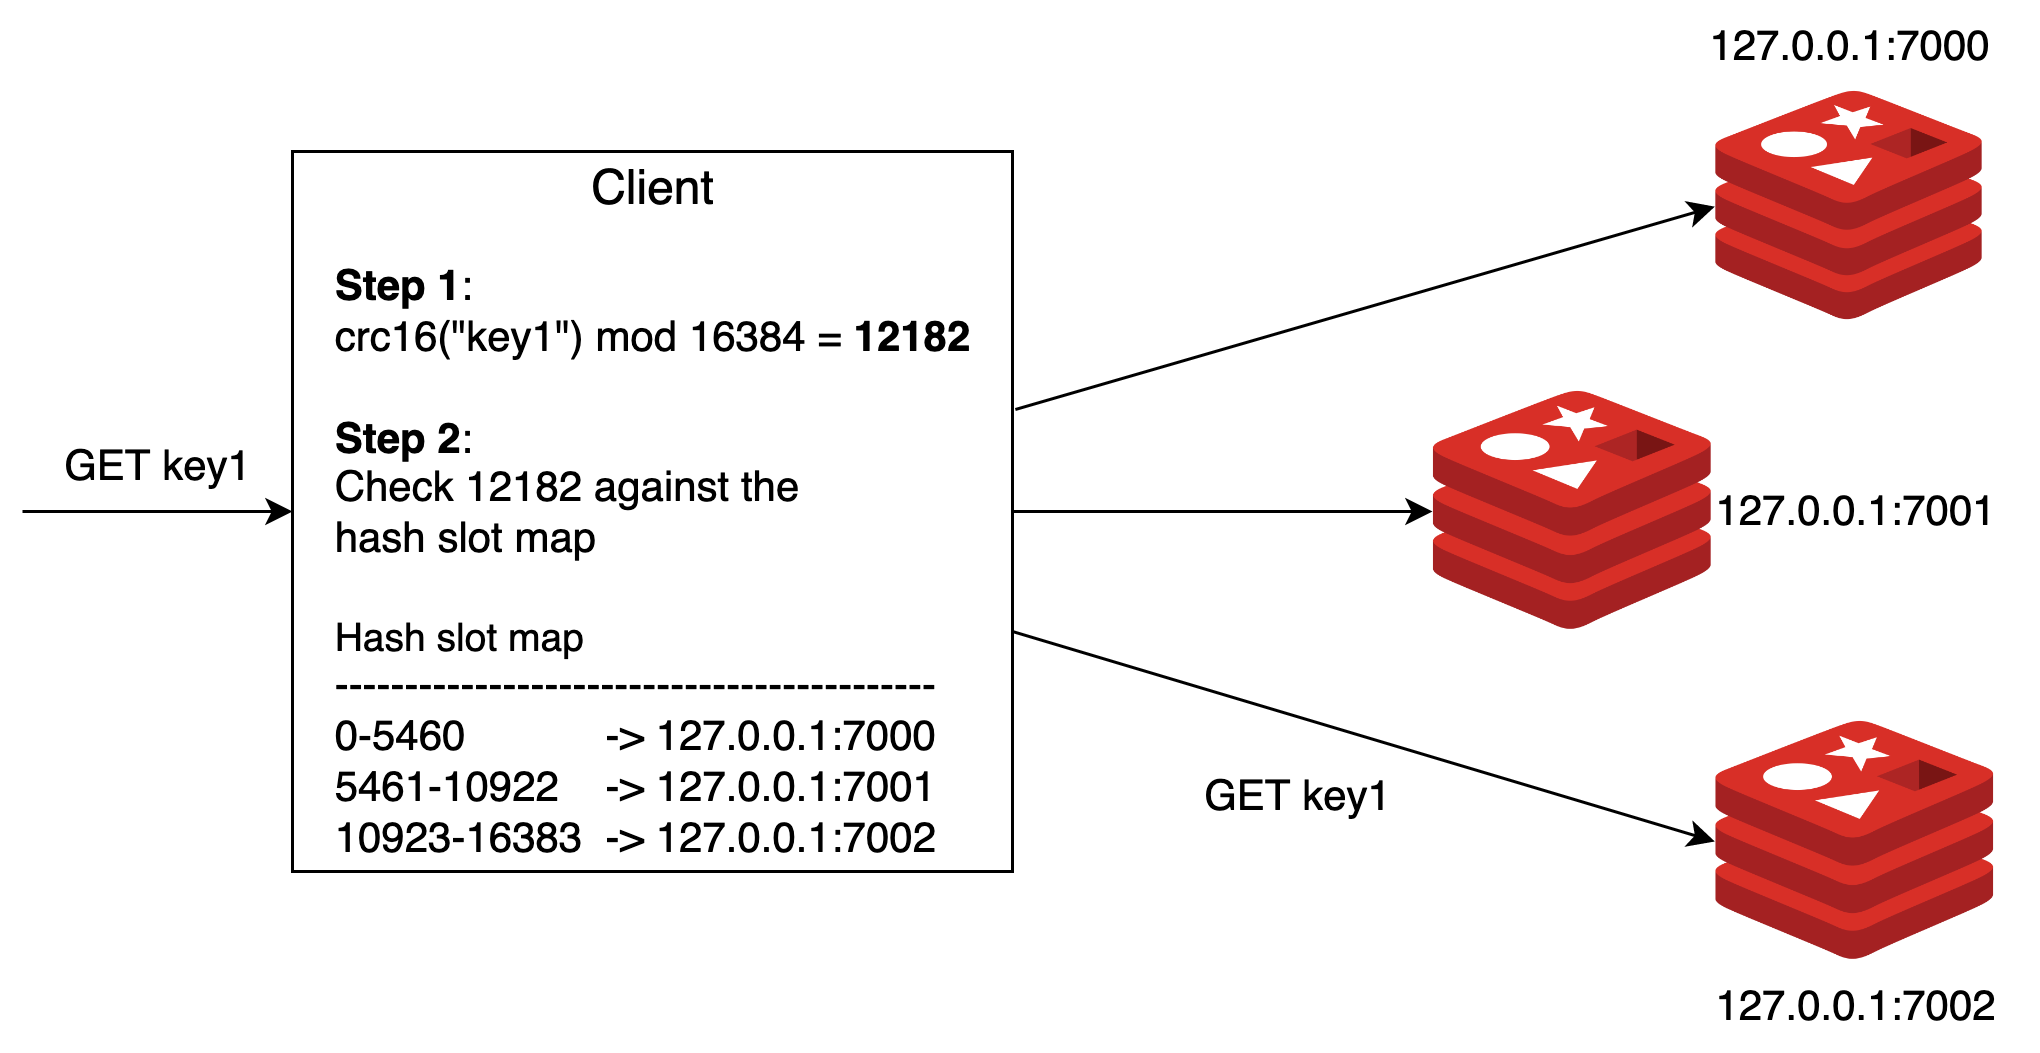
\includegraphics[width=0.9\textwidth]{img/hashslotCluster}
    \end{center}
\caption{Redis distribuito Cluster}
\end{figure}\\
\\
Lo sharding dei dati in molte istanze non risolve il problema della sicurezza dei dati e della ridondanza. Se una delle istanze muore
a causa di un guasto hardware e non si hanno backup da cui ripristinare i dati, tutti i dati di quella istanza saranno persi.
Per evitare, o quanto meno diminuire, questo problema si potrebbero utilizzare diverse tecniche, come la replicazione su disco oppure l'architettura master-slave.\\
Inoltre, le transazioni relative a piú chiavi distribuite su piú istanze non sono supportate, poiché richiederebbero lo spostamento
dei dati tra diversi nodi, con conseguente calo delle prestazioni.\\
\\


\begin{figure}[H]
    \begin{center}
        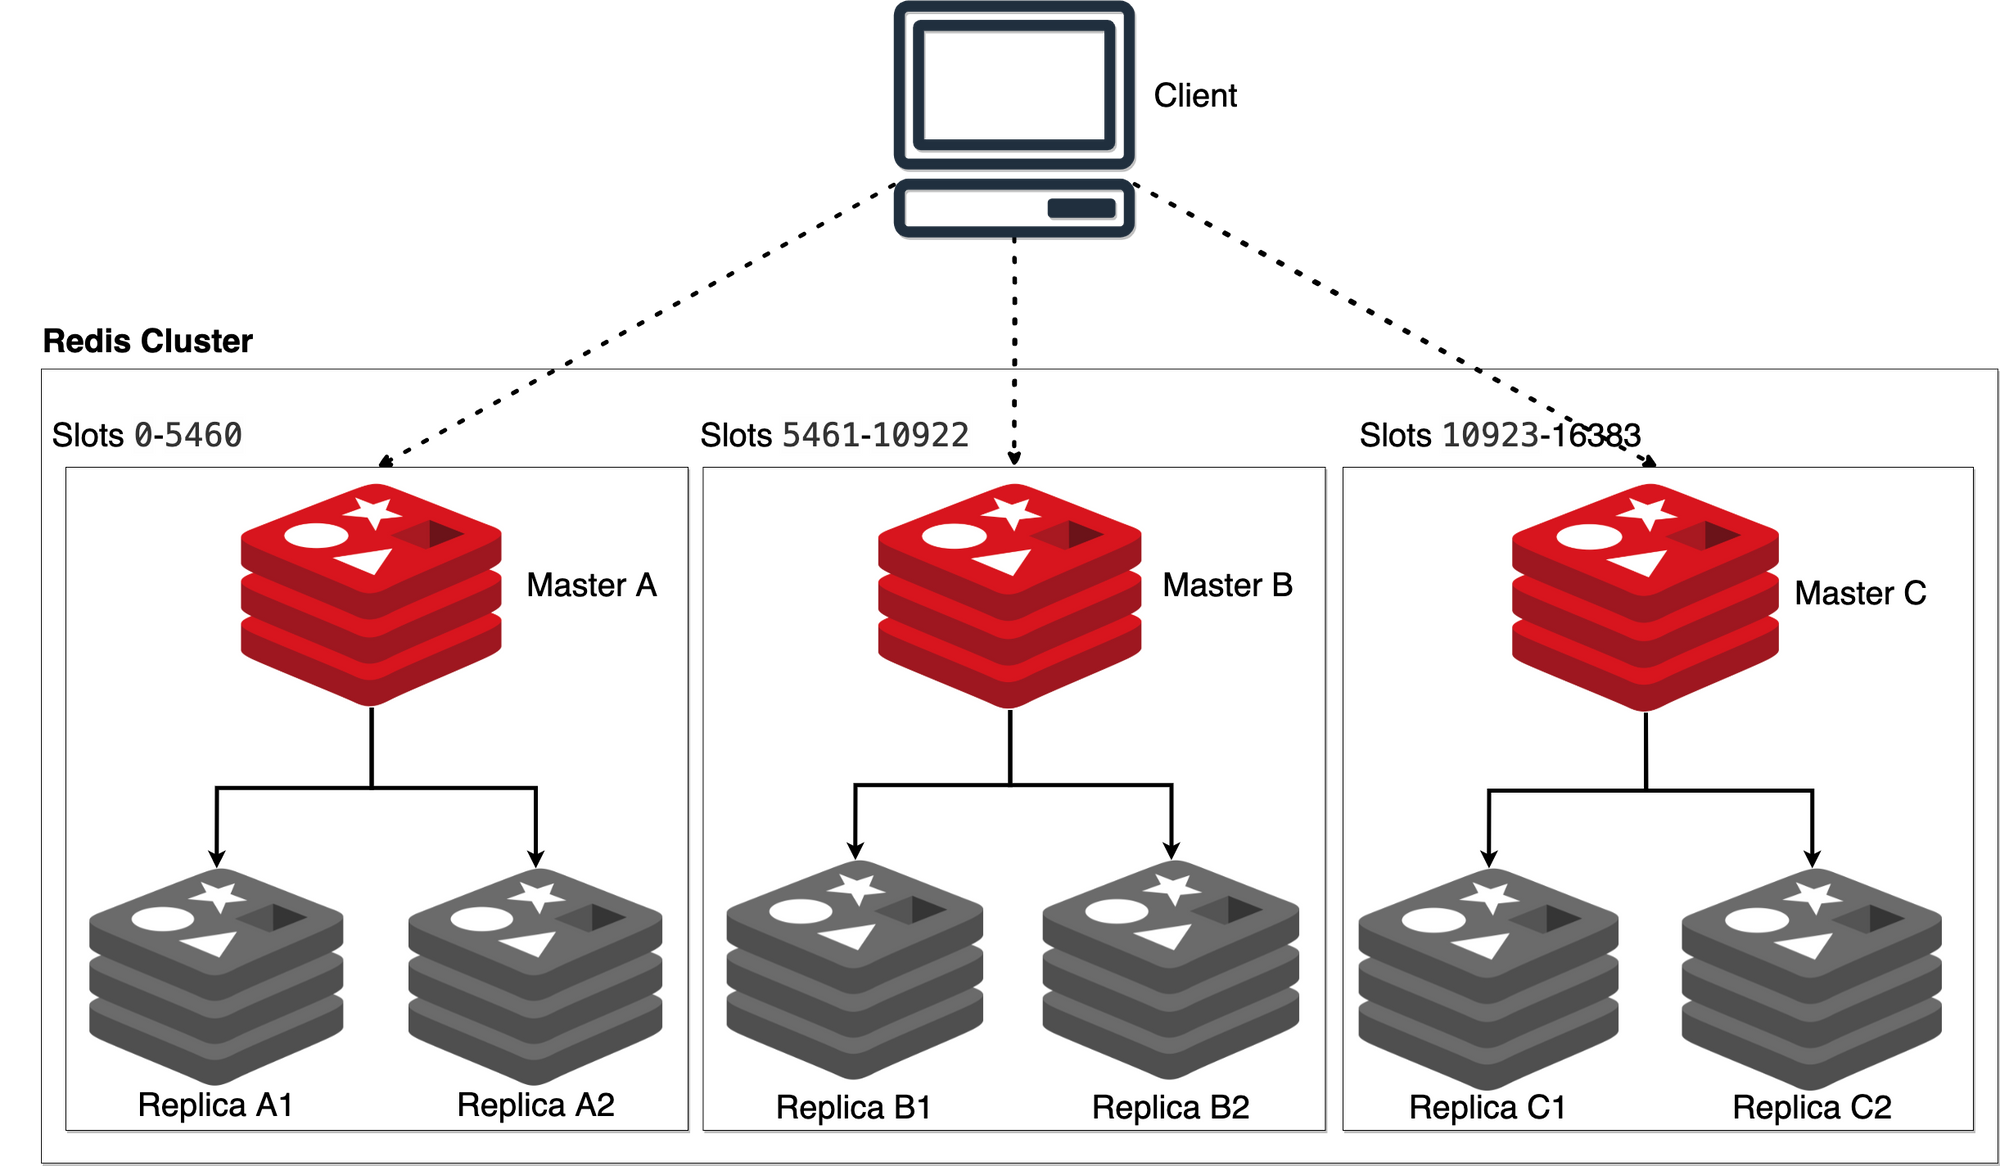
\includegraphics[width=0.9\textwidth]{img/cluster:master-slaveRedis}
    \end{center}
    \label{clusterMasterSlave}
\caption{Redis distribuito avanzato con Cluster e Master-Slave}
\end{figure}
La Figura mostra un sistema avanzato in cui si ha una combinazione di Redis Cluster e Redis Master-Slave.